\chapter{Análisis}

En este capítulo se define el marco conceptual y funcional del videojuego, estableciendo las bases operativas necesarias para el posterior diseño técnico. En primer lugar, se delimitan los actores y se detallan los requisitos funcionales, no funcionales y de información que gobiernan el sistema. Posteriormente, se especifican los casos de uso a través de sus flujos normales y alternativos para describir detalladamente el comportamiento de la aplicación. Por último, se presenta el modelo de dominio con las entidades clave del juego y se analizan los procesos de negocio mediante diagramas de actividad, ofreciendo una visión dinámica de los turnos, combates y fases del desarrollo de la partida.

% ─────────────────────────────────────────────────────────────────────────────
\section{Actores y roles}
% ─────────────────────────────────────────────────────────────────────────────

En este apartado se identifican los actores que interactúan con el Sistema, entendiendo como actor toda entidad externa que inicia o participa en la ejecución de casos de uso.

El único actor del sistema es el \textbf{Jugador}, que corresponde a la persona que interactúa con el videojuego a través de la interfaz gráfica mediante el ratón. Es el actor principal y exclusivo, responsable de iniciar y configurar la partida, desplegar sus piezas en la fase inicial, realizar movimientos y ataques durante su turno, y pausar o abandonar la partida en cualquier momento. El resto de la lógica del videojuego, incluyendo las acciones del oponente, es gestionada internamente por el propio sistema sin intervención externa.

\clearpage

% ─────────────────────────────────────────────────────────────────────────────
\section{Modelado de Requisitos}
% ─────────────────────────────────────────────────────────────────────────────

Los requisitos describen las condiciones, capacidades y restricciones que debe cumplir un sistema software para satisfacer las necesidades de sus usuarios y los objetivos de la organización. Se distinguen principalmente tres tipos de requisitos: los requisitos funcionales (RF), que especifican los servicios y comportamientos que debe ofrecer el sistema; los requisitos no funcionales (RNF), que establecen restricciones y propiedades de calidad como rendimiento, fiabilidad o usabilidad; y los requisitos de información (RI), que definen los datos que el sistema debe almacenar y gestionar para proporcionar dichos servicios.

\subsection{Requisitos funcionales}

\begin{itemize}
	
	\item \textbf{RF01:} El Sistema permitirá iniciar una nueva partida desde un estado inicial controlado, inicializando el tablero, las piezas y el turno inicial conforme a las reglas del videojuego.
	
	\item \textbf{RF02:} El Sistema permitirá al Jugador colocar sus piezas al inicio de la partida dentro de la zona de despliegue definida.
	
	\item \textbf{RF03:} El Sistema gestionará los turnos alternos entre el Jugador y el bot, impidiendo la realización de acciones fuera de turno.
	
	\item \textbf{RF04:} El Sistema validará las acciones realizadas por el Jugador, evitando movimientos o ataques no permitidos por las	reglas del videojuego.
	
	\item \textbf{RF05:} El Sistema revelará la identidad de las piezas implicadas cuando se produzca un combate o movimiento característico, manteniendo visible la información revelada durante el resto de la partida.
	
	\item \textbf{RF06:} El Sistema hará que el bot tome las decisiones de movimiento y ataque de forma autónoma durante su turno, respetando las reglas y restricciones del videojuego.
	
	\item \textbf{RF07:} El Sistema mantendrá y actualizará el estado de la partida durante su desarrollo, gestionando turnos, acciones válidas y transiciones entre estados.
	
	\item \textbf{RF08:} El Sistema determinará automáticamente el final de la partida cuando se cumpla una condición de victoria o derrota, mostrando el resultado al Jugador.
	
	\item \textbf{RF09:} El Sistema mostrará información visual y sonora relacionada con las acciones realizadas, los combates y los cambios de estado de la partida.
	
	\item \textbf{RF10:} El Sistema permitirá al Jugador pausar o abandonar la partida en curso de forma controlada.
	
	\item \textbf{RF11:} El Sistema brindará al Jugador con la información necesaria para entender las reglas del videojuego en caso de no conocerlas.
	
	\item \textbf{RF12:} El Sistema permitirá al Jugador configurar los parámetros de audio del videojuego (volumen de música, efectos de sonido, etc.) desde el menú de opciones antes y durante una partida.
	
\end{itemize}

\subsection{Requisitos no funcionales}
\begin{itemize}
	
	\item \textbf{RNF01:} El sistema deberá ser compatible con Windows 10, Windows 11, y distribuciones de Linux lanzadas a partir de 2018.
	
	\item \textbf{RNF02:} El videojuego deberá ejecutarse correctamente en un equipo con las siguientes especificaciones mínimas de hardware:
	\begin{itemize}
		\item Procesador: CPU de doble núcleo a 2,0~GHz o superior.
		\item Memoria RAM: 4~GB.
		\item Tarjeta gráfica: GPU con soporte completo de Vulkan~1.0 (por ejemplo, Intel HD Graphics 510 o superior).
		\item Almacenamiento: 200~MB de espacio libre en disco.
	\end{itemize}
	
	\item \textbf{RNF03:} El sistema deberá responder a las acciones del jugador en un tiempo máximo de 2 segundos en condiciones normales de ejecución, garantizando una experiencia de juego fluida.
	
	\item \textbf{RNF04:} La interfaz deberá ser suficientemente clara e intuitiva para que un jugador sin experiencia previa en el videojuego pueda comprender las acciones disponibles en cada momento sin necesidad de consultar las reglas.
	
	\item \textbf{RNF05:} La interfaz del videojuego será completamente manejable mediante ratón.
	
\end{itemize}

\subsection{Requisitos de información}

\begin{itemize}
	\item \textbf{RI01 --- Partida:} El Sistema gestionará una sesión de juego con la siguiente información:
	\begin{itemize}
		\item Referencia al tablero de juego.
		\item Turno actual (Jugador o Bot).
		\item Estado de la partida (Fase de despliegue, turno del Jugador, pieza seleccionada y fin de la partida).
		\item Número de turno.
		\item Conjunto de casillas que conforman el tablero.
	\end{itemize}
	
	\item \textbf{RI02 --- Casilla:} Cada casilla del tablero almacenará la siguiente información:
	\begin{itemize}
		\item Posición en la cuadrícula $(x, y)$.
		\item Tipo (Pasable, no pasable, despliegue del Jugador y del bot).
		\item Pieza que la ocupa, si la	hubiera.
	\end{itemize}
	
\clearpage

	\item \textbf{RI03 --- Pieza:} El Sistema almacenará la siguiente información para cada pieza presente en la partida:
	\begin{itemize}
		\item Tipo de pieza (Los 12 tipos de piezas que vienen recogidos en el capítulo de Diseño del videojuego).
		\item Rango numérico que determina el resultado de los combates.
		\item Propietario (Jugador o Bot).
		\item Si la pieza puede moverse o no.
		\item Si es visible para el Jugador.
		\item Si el bot conoce la identidad de la pieza.
		\item Casilla del tablero en la que se situa.
		\item Historial de los últimos tres movimientos realizados como origen-destino.
	\end{itemize}
\end{itemize}

% ─────────────────────────────────────────────────────────────────────────────
\section{Casos de uso}
% ─────────────────────────────────────────────────────────────────────────────

En este apartado se describen los casos de uso del Sistema, que representan las interacciones posibles entre el actor y el Sistema para alcanzar un objetivo concreto. Cada caso de uso recoge el flujo normal de acciones, las posibles excepciones y los requisitos funcionales asociados. La Figura~\ref{fig:diagrama_cu} muestra el diagrama general de casos de uso, donde se reflejan las relaciones entre el actor, los casos de uso principales y las dependencias entre ellos.

\begin{figure}[H]
	\centering
	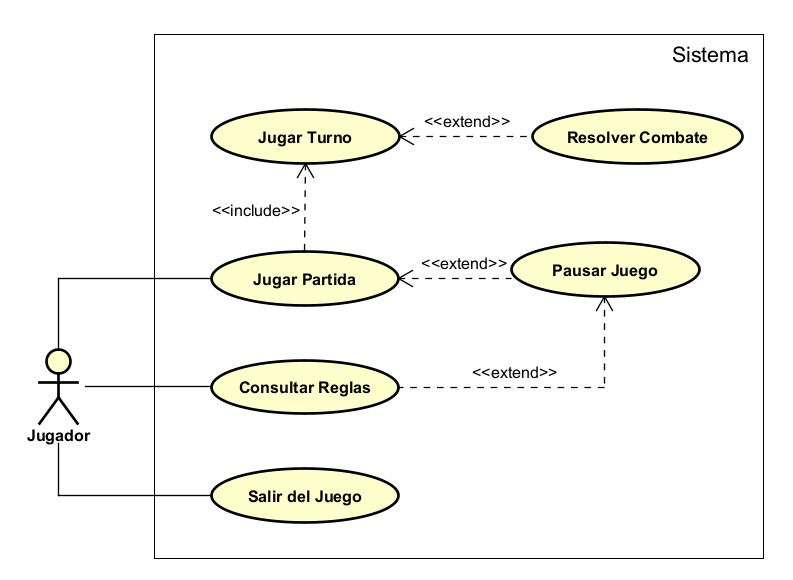
\includegraphics[width=\linewidth]{../Imagenes/DiagramaCasosDeUso}
	\caption{Diagrama de casos de uso}
	\label{fig:diagrama_cu}
\end{figure}

\clearpage

\subsection{Lista de casos de uso}

\begin{table}[H]
	\centering
	\begin{tabular}{|p{1.2cm}|p{4.2cm}|p{11cm}|}
		\hline
		\textbf{ID} & \textbf{Nombre} & \textbf{Descripción} \\
		\hline CU-01 & Iniciar partida & El Sistema permite al Jugador iniciar una nueva partida. \\
		\hline CU-02 & Jugar ronda & El Sistema permite al Jugador llevar a cabo un turno completo durante el transcurso de una partida. \\
		\hline CU-03 & Resolver combate & El Sistema gestiona el combate entre 2 piezas de manera automática. \\
		\hline CU-04 & Pausar partida & El Sistema permitirá al Jugador pausar en mitad de una partida cuando sea su turno. \\
		\hline CU-05 & Abandonar partida & El Sistema permitirá al Jugador salir durante el transcurso de una partida cuando sea su turno. \\
		\hline CU-06 & Consultar reglas & El Sistema permite al Jugador consultar las reglas dentro del videojuego. \\
		\hline CU-07 & Consultar opciones & El Sistema permite al Jugador consultar y configurar las opciones. \\
		\hline
	\end{tabular}
	\caption{Lista de casos de uso del Sistema}
	\label{tab:casosdeuso}
\end{table}

% ─────────────────────────────────────────────────────────────────────────────

\subsection{CU-01: Iniciar partida}

\begin{table}[H]
	\centering
	\begin{tabular}{|p{3cm}|p{14cm}|}
		\hline \textbf{ID} & CU-01 \\
		\hline \textbf{Nombre} & Iniciar partida \\
		\hline \textbf{Actor} & Jugador \\
		\hline \textbf{Descripción} & El Sistema permite al Jugador iniciar una nueva partida. \\
		\hline \textbf{Req. relacionados} & RF01, RF02.\\
		\hline \textbf{Pre-condición} & El Sistema se encuentra mostrando la escena del menú principal, o la del final de partida.\\
		\hline
		\textbf{Secuencia normal} &
		\begin{enumerate}[nosep, before=\vspace{-0.4\baselineskip}]
			\item El Jugador selecciona la opción de jugar una partida.
			\item El Sistema inicia el tablero y espera a que el Jugador distribuya sus piezas en su zona.
			\item El Jugador coloca todas sus piezas en el tablero.
			\item El Jugador solicita comenzar la partida.
			\item El Sistema distribuye todas las piezas del bot e inicia la partida.
		\end{enumerate} \\
		\hline
		\textbf{Flujos alternativos} &
		\begin{itemize}[nosep, before=\vspace{-0.4\baselineskip}]
			\item [{3.a.}] El Jugador solicita pausar el juego → Se inicia CU-04 (Pausar partida).
			\item [{4.a.}] No están todas las piezas colocadas → Regresa al paso 3.
		\end{itemize} \\
		\hline \textbf{Post-condición} & La partida comienza con el primer turno el cual espera acción del Jugador. \\
		\hline
	\end{tabular}
	\caption{CU-01: Iniciar partida}
	\label{tab:cu01}
\end{table}

\clearpage

% ─────────────────────────────────────────────────────────────────────────────

\subsection{CU-02: Jugar ronda}

\begin{table}[H]
	\centering
	\begin{tabular}{|p{3cm}|p{14cm}|}
		\hline \textbf{ID} & CU-02 \\
		\hline \textbf{Nombre} & Jugar ronda \\
		\hline \textbf{Actor} & Jugador \\
		\hline \textbf{Descripción} & El Sistema permite al Jugador llevar a cabo un turno completo durante el transcurso de una partida. \\
		\hline \textbf{Req. relacionados} & RF03, RF04, RF05, RF06, RF07, RF08, RF09, RF10. \\
		\hline \textbf{Pre-condición} & El Jugador se encuentra jugando a mitad de una partida y es su turno. \\
		\hline
		\textbf{Secuencia normal} &
		\begin{enumerate}[nosep, before=\vspace{-0.4\baselineskip}]
			\item El Jugador solicita mover una de sus piezas.
			\item El Sistema realiza la acción solicitada por el Jugador.
			\item El Sistema cede el turno al bot.
			\item El Sistema ejecuta el turno del bot, realizando una acción valida con una de sus piezas.
			\item El Sistema cede el turno al Jugador.
		\end{enumerate} \\
		\hline
		\textbf{Flujos alternativos} &
		\begin{itemize}[nosep, before=\vspace{-0.4\baselineskip}]
			\item [{1.a.}] El Jugador no puede mover ninguna pieza → el Sistema termina la partida y el caso de uso finaliza.
			\item [{1.b.}] El Jugador solicita hacer un movimiento inválido → el Sistema ignora la acción y regresa al paso 1.
			\item [{1.c.}] El Jugador solicita pausar la partida → Se inicia CU-04 (Pausar partida), y una vez terminado el caso de uso continua.
			\item [{2.a.}] La pieza se ha movido a una casilla vacía con un movimiento característico → El Sistema revela la identidad de esa pieza y el caso de uso continua.
			\item [{2.b.}] La casilla destino esta ocupada por una pieza del bot → Se inicia CU-03 (Resolver combate), y una vez terminado el caso de uso continua.
			\item [{3.a.}] Tras la acción del Jugador se da una condición para finalizar la partida → El Sistema termina la partida y el caso de uso finaliza.
			\item [{4.a.}] La pieza se ha movido a una casilla vacía con un movimiento característico → El Sistema revela la identidad de esa pieza y el caso de uso continua.
			\item [{4.b.}] La casilla destino esta ocupada por una pieza del Jugador → Se inicia CU-03 (Resolver combate), y una vez terminado el caso de uso continua.
			\item [{5.a.}] Tras la acción del bot se da una condición para finalizar la partida → El Sistema termina la partida y el caso de uso finaliza.
		\end{itemize} \\
		\hline \textbf{Post-condición} & N/A \\
		\hline
	\end{tabular}
	\caption{CU-02: Jugar ronda}
	\label{tab:cu02}
\end{table}

\clearpage

% ─────────────────────────────────────────────────────────────────────────────

\subsection{CU-03: Resolver combate}

\begin{table}[H]
	\centering
	\begin{tabular}{|p{3cm}|p{14cm}|}
		\hline \textbf{ID} & CU-03 \\
		\hline \textbf{Nombre} & Resolver combate \\
		\hline \textbf{Actor} & Jugador \\
		\hline \textbf{Descripción} & El Sistema gestiona el combate entre 2 piezas de manera automática. \\
		\hline \textbf{Req. relacionados} & RF05, RF09. \\
		\hline \textbf{Pre-condición} & Durante una partida en curso, se ha movido una pieza a una casilla ocupada por otra pieza del bando rival. \\
		\hline
		\textbf{Secuencia normal} &
		\begin{enumerate}[nosep, before=\vspace{-0.4\baselineskip}]
			\item El Sistema revela las piezas que entran en combate.
			\item El Sistema lleva a cabo el combate y obtiene el resultado según las reglas.
			\item El Jugador conoce el resultado y solicita continuar con la partida.
			\item El Sistema elimina del tablero la pieza que resulta perdedora del combate. En caso de que pierdan ambas piezas se eliminan ambas.
		\end{enumerate} \\
		\hline
		\textbf{Flujos alternativos} &
		\begin{itemize}[nosep, before=\vspace{-0.4\baselineskip}]
			\item [{1.a.}] No hay piezas ocultas → El Sistema ignora este paso y continua al paso 2.
		\end{itemize} \\
		\hline \textbf{Post-condición} & N/A \\
		\hline
	\end{tabular}
	\caption{CU-03: Resolver combate}
	\label{tab:cu03}
\end{table}

\clearpage

% ─────────────────────────────────────────────────────────────────────────────

\subsection{CU-04: Pausar partida}

\begin{table}[H]
	\centering
	\begin{tabular}{|p{3cm}|p{14cm}|}
		\hline \textbf{ID} & CU-04 \\
		\hline \textbf{Nombre} & Pausar partida \\
		\hline \textbf{Actor} & Jugador \\
		\hline \textbf{Descripción} & El Sistema permitirá al Jugador pausar en mitad de una partida cuando sea su turno. \\
		\hline \textbf{Req. relacionados} & RF10. \\
		\hline \textbf{Pre-condición} & El Jugador se encuentra jugando su turno en el transcurso de una partida. \\
		\hline
		\textbf{Secuencia normal} &
		\begin{enumerate}[nosep, before=\vspace{-0.4\baselineskip}]
			\item El Jugador solicita pausar la partida.
			\item El Sistema pausa la partida.
			\item El Jugador decide continuar con la partida.
			\item El Sistema permite al Jugador continuar con la partida.
		\end{enumerate} \\
		\hline
		\textbf{Flujos alternativos} &
		\begin{itemize}[nosep, before=\vspace{-0.4\baselineskip}]
			\item [{1.a.}] El Jugador decide consultar las reglas → Se inicia CU-06 (Consultar reglas), y una vez terminado el caso de uso continua.
			\item [{1.b.}] El Jugador decide consultar las opciones → Se inicia CU-07 (Consultar opciones), y una vez terminado el caso de uso continua.
			\item [{1.c.}] El Jugador decide abandonar la partida → Se inicia CU-05 (Abandonar partida), y el caso de uso finaliza.
		\end{itemize} \\
		\hline \textbf{Post-condición} & N/A \\
		\hline
	\end{tabular}
	\caption{CU-04: Pausar partida}
	\label{tab:cu04}
\end{table}

\clearpage

% ─────────────────────────────────────────────────────────────────────────────

\subsection{CU-05: Abandonar partida}

\begin{table}[H]
	\centering
	\begin{tabular}{|p{3cm}|p{14cm}|}
		\hline \textbf{ID} & CU-05 \\
		\hline \textbf{Nombre} & Abandonar partida \\
		\hline \textbf{Actor} & Jugador \\
		\hline \textbf{Descripción} & El Sistema permitirá al Jugador salir durante el transcurso de una partida cuando sea su turno. \\
		\hline \textbf{Req. relacionados} & RF10. \\
		\hline \textbf{Pre-condición} & El Jugador está en una partida actualmente pausada. \\
		\hline
		\textbf{Secuencia normal} &
		\begin{enumerate}[nosep, before=\vspace{-0.4\baselineskip}]
			\item El Jugador solicita abandonar la partida.
			\item El Sistema finaliza la partida.
		\end{enumerate} \\
		\hline
		\textbf{Flujos alternativos} &
		\begin{itemize}[nosep, before=\vspace{-0.4\baselineskip}]
			\item N/A
		\end{itemize} \\
		\hline \textbf{Post-condición} & N/A \\
		\hline
	\end{tabular}
	\caption{CU-05: Abandonar partida}
	\label{tab:cu05}
\end{table}

% ─────────────────────────────────────────────────────────────────────────────

\subsection{CU-06: Consultar reglas}

\begin{table}[H]
	\centering
	\begin{tabular}{|p{3cm}|p{14cm}|}
		\hline \textbf{ID} & CU-06 \\
		\hline \textbf{Nombre} & Consultar reglas \\
		\hline \textbf{Actor} & Jugador \\
		\hline \textbf{Descripción} & El Sistema permite al Jugador consultar las reglas dentro del videojuego. \\
		\hline \textbf{Req. relacionados} & RF11. \\
		\hline \textbf{Pre-condición} & N/A \\
		\hline
		\textbf{Secuencia normal} &
		\begin{enumerate}[nosep, before=\vspace{-0.4\baselineskip}]
			\item El Jugador solicita consultar las reglas del videojuego.
			\item El Sistema da a conocer las reglas al Jugador.
		\end{enumerate} \\
		\hline
		\textbf{Flujos alternativos} &
		\begin{itemize}[nosep, before=\vspace{-0.4\baselineskip}]
			\item N/A
		\end{itemize} \\
		\hline \textbf{Post-condición} & N/A \\
		\hline
	\end{tabular}
	\caption{CU-06: Consultar reglas}
	\label{tab:cu06}
\end{table}

\clearpage

% ─────────────────────────────────────────────────────────────────────────────

\subsection{CU-07: Consultar opciones}

\begin{table}[H]
	\centering
	\begin{tabular}{|p{3cm}|p{14cm}|}
		\hline \textbf{ID} & CU-07 \\
		\hline \textbf{Nombre} & Consultar opciones \\
		\hline \textbf{Actor} & Jugador \\
		\hline \textbf{Descripción} & El Sistema permite al Jugador consultar y configurar las opciones. \\
		\hline \textbf{Req. relacionados} & RF12. \\
		\hline \textbf{Pre-condición} & N/A \\
		\hline
		\textbf{Secuencia normal} &
		\begin{enumerate}[nosep, before=\vspace{-0.4\baselineskip}]
			\item El Jugador solicita configurar las opciones del videojuego.
			\item El Sistema permite al Jugador modificar las distintas opciones de manera controlada.
		\end{enumerate} \\
		\hline
		\textbf{Flujos alternativos} &
		\begin{itemize}[nosep, before=\vspace{-0.4\baselineskip}]
			\item N/A
		\end{itemize} \\
		\hline \textbf{Post-condición} & N/A \\
		\hline
	\end{tabular}
	\caption{CU-07: Consultar opciones}
	\label{tab:cu07}
\end{table}

\clearpage

% ─────────────────────────────────────────────────────────────────────────────
\section{Modelo de dominio}
% ─────────────────────────────────────────────────────────────────────────────

El modelo de dominio es una representación visual de las entidades conceptuales (objetos del mundo real o del Sistema) y las relaciones que existen entre ellas dentro del contexto del videojuego. Su objetivo es identificar los conceptos clave, sus atributos y cómo interactúan, sirviendo como puente entre los requisitos funcionales y el diseño técnico final.

A continuación, en la Figura~\ref{fig:modelo_dominio}, se presenta el modelo de dominio que estructura la lógica del videojuego.

\begin{figure}[H]
	\centering
	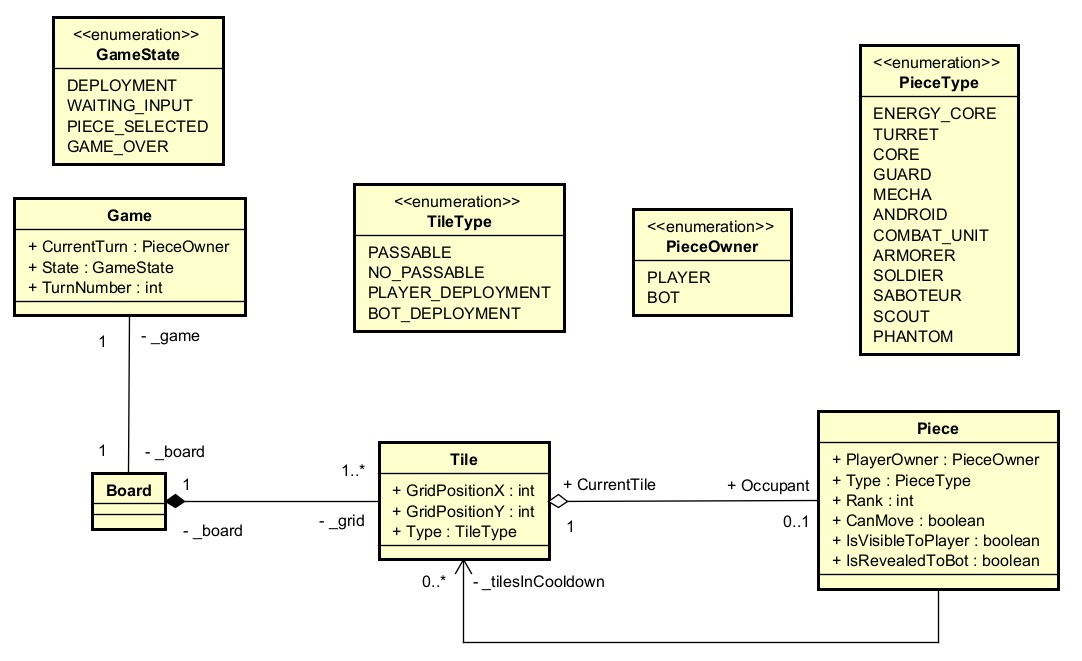
\includegraphics[width=\linewidth]{../Imagenes/DiagramaModeloDominio}
	\caption{Diagrama del modelo de dominio}
	\label{fig:modelo_dominio}
\end{figure}

\clearpage

% ─────────────────────────────────────────────────────────────────────────────
\section{Modelo de proceso de negocio}
% ─────────────────────────────────────────────────────────────────────────────

El modelo de proceso de negocio describe el flujo detallado de actividades y decisiones que tienen lugar durante la ejecución del Sistema. Mientras que los casos de uso definen \textit{qué} hace el Sistema, los diagramas de actividad reflejan \textit{cómo} se ejecutan dichas interacciones, mostrando la secuencia lógica, las bifurcaciones y el procesamiento de datos.

A continuación, se detallan los flujos de actividad correspondientes a los casos de uso mas importantes del Sistema, proporcionando una visión dinámica de la lógica del videojuego.

\subsection{Actividad: Iniciar partida}

El diagrama de actividad de la Figura~\ref{fig:DiagramaActividadIniciarPartida} representa el CU-01 (Iniciar Partida), que transcurre de forma que el Jugador decide iniciar una nueva partida, el Sistema instancia las piezas con su identidad oculta para el rival, tanto del Jugador según las va colocando, como las del bot cuando el Jugador solicita iniciar la partida.

\begin{figure}[H]
	\centering
	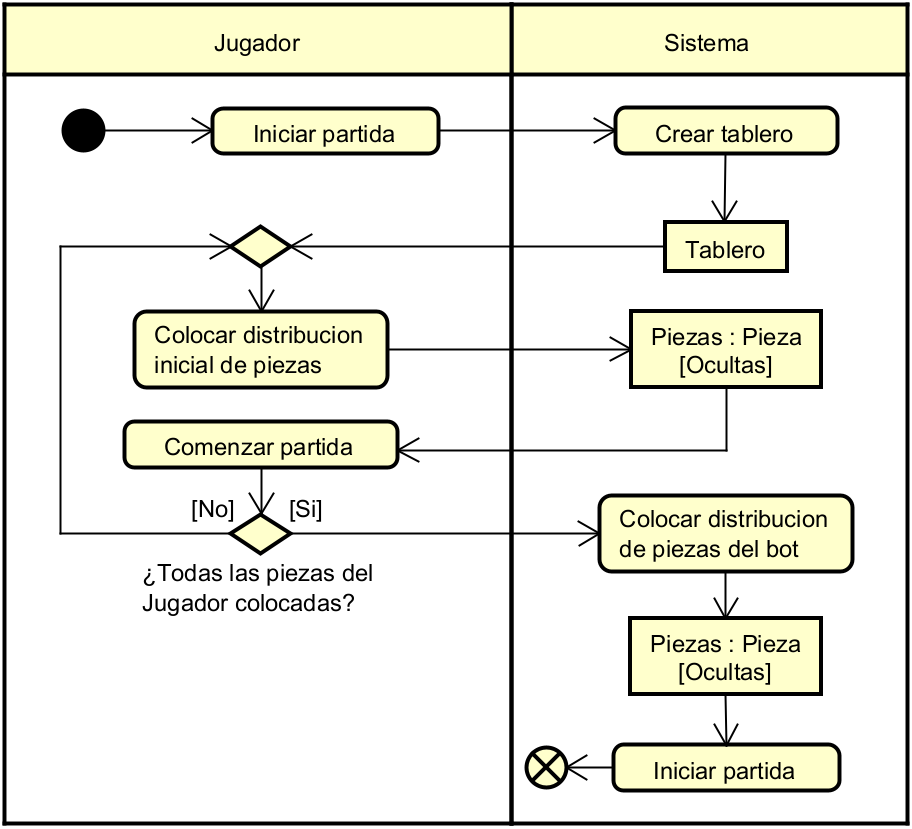
\includegraphics[width=0.9\linewidth]{../Imagenes/DiagramaActividadIniciarPartida}
	\caption{Diagrama de actividad: Iniciar partida}
	\label{fig:DiagramaActividadIniciarPartida}
\end{figure}

\clearpage

\subsection{Actividad: Jugar ronda}

El diagrama de actividad que se muestra en la Figura~\ref{fig:DiagramaActividadJugarTurno}, representa el CU-02 (Jugar ronda), en el cual se puede ver el transcurso del turno del jugador y del bot. Desde un movimiento de pieza normal, uno peculiar que revela la identidad de una pieza, o un movimiento que acaba en la casilla de una pieza rival y se disputa un combate entre ambas piezas.

\begin{figure}[H]
	\centering
	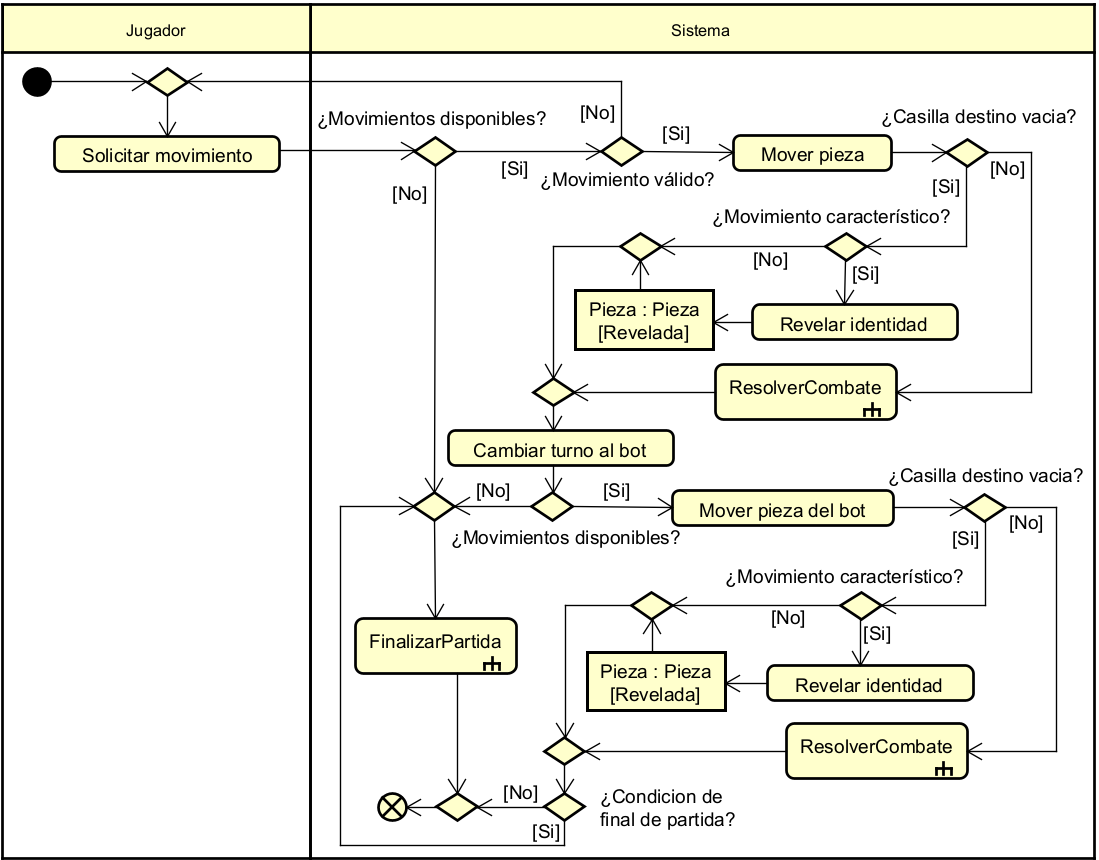
\includegraphics[width=\linewidth]{../Imagenes/DiagramaActividadJugarTurno}
	\caption{Diagrama de actividad: Jugar ronda}
	\label{fig:DiagramaActividadJugarTurno}
\end{figure}

\clearpage

\subsection{Actividad: Resolver combate}

El diagrama de la Figura~\ref{fig:DiagramaActividadResolverCombate} muestra el transcurso de un combate entre 2 piezas. Siempre que una pieza entra a combate queda revelada, y aquella que pierde según las reglas del videojuego, es eliminada. En caso de empate ambas se eliminan.

\begin{figure}[H]
	\centering
	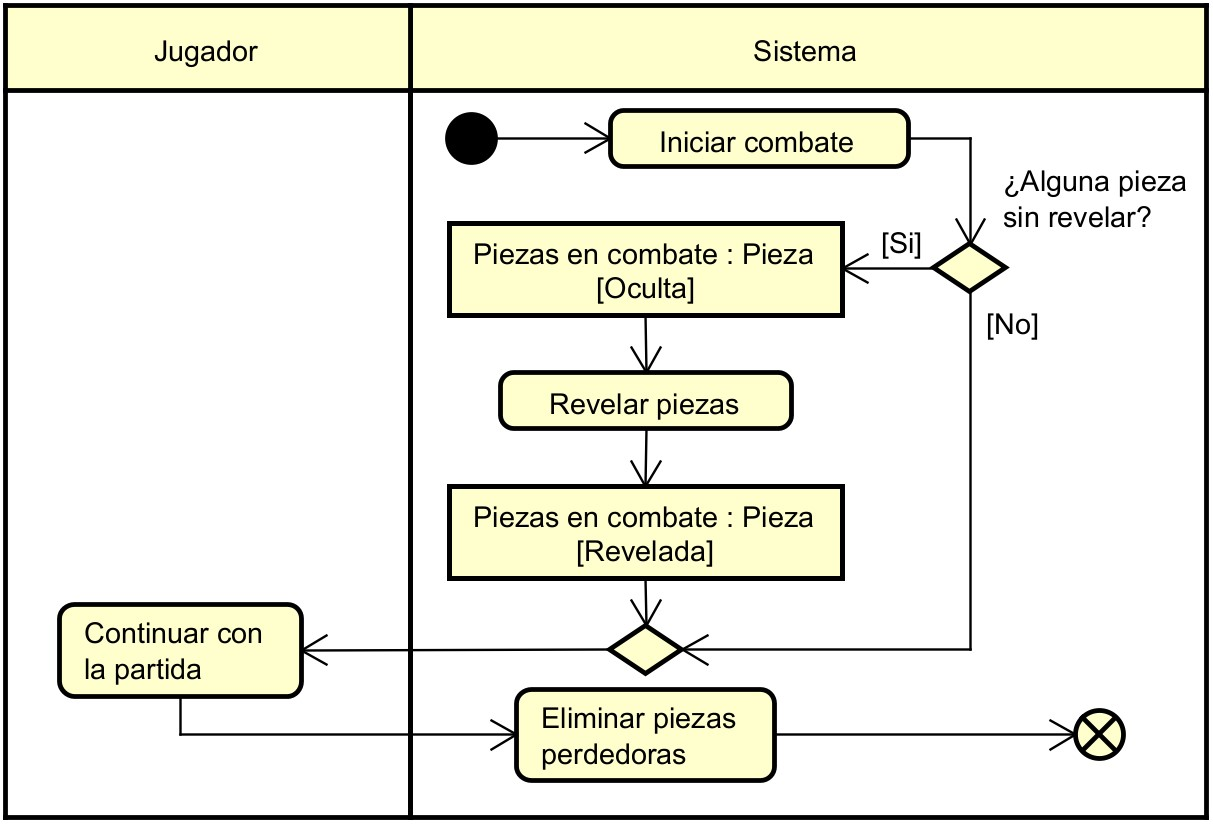
\includegraphics[width=\linewidth]{../Imagenes/DiagramaActividadResolverCombate}
	\caption{Diagrama de actividad: Resolver combate}
	\label{fig:DiagramaActividadResolverCombate}
\end{figure}